\chapter{微分学基础}\label{chap:calculus}
本书中的积分学使用非常少,并且集中在概率论部分,所以在本附录中我们只讨论微分学,积分学的内容在概率论中简单介绍. 尽管我们的视角非常一般且抽象,我们主要讨论的是Euclid空间$\R^n$相关的微分学. 

\section{点集拓扑}\label{sec:topology}
本部分讨论极限、连续、紧致等概念,这些概念是微分学的基础. 

\subsection{度量空间,范数}\label{subsec:metric-norm}
实数集$\R$上面的元素可以被看成一些点,这些点之间有距离的概念. 这是$\R$最重要的几个性质之一. 我们把这种性质抽象出来,得到度量空间的概念. 

\begin{definition}[度量空间]\index{度量空间}\index{度量}
设$X$是一个集合,$d:X\times X\to\R$是一个函数,如果满足
\begin{enumerate}
    \item 非负性:对任意$x,y\in X$,$d(x,y)\geq 0$,且$d(x,y)=0$当且仅当$x=y$;
    \item 对称性:对任意$x,y\in X$,$d(x,y)=d(y,x)$;
    \item 三角不等式:对任意$x,y,z\in X$,$d(x,z)\leq d(x,y)+d(y,z)$. 
\end{enumerate}
则称$(X,d)$是一个\textbf{度量空间},$d$称为\textbf{度量}. 
\end{definition}

下面给出一些度量的例子,但我们不给出验证. 
\begin{example}\label{ex:metric}
    考虑实数集$\R$,要成为度量空间,可以装备以下度量:
    \begin{itemize}
            \item 平凡的离散度量:$\forall x_1\neq x_2\ d(x_1,x_2)\equiv 1, d(x,x)=0$. \index{度量!离散~}
            \item $d(x_1,x_2)=|x_1-x_2|$. \index{度量!绝对值~}
        \end{itemize}
        考虑向量空间$\R^n$,要成为度量空间,可以装备以下度量:
        \begin{itemize}
            \item Minkowski度量($L^p$度量):$d(x_1,x_2)=(\sum_{i=1}^n|x_1^i-x_2^i|^p)^{1/p}\ (p\ge 1)$. \index{度量!Minkowski~}\index{度量!$L^p$~}
            \item Manhattan度量($L^1$度量): $d(x_1,x_2)=\sum_{i=1}^n|x_1^i-x_2^i|$. \index{度量!Manhattan~}\index{度量!$L^1$~}
            \item Euclid度量($L^2$度量):$d(x_1,x_2)=\sqrt{\sum_{i=1}^n|x_1^i-x_2^i|^2}$. \index{度量!Euclid~}\index{度量!$L^2$~}
            \item Chebyshev度量($L^\infty$度量): $d(x_1,x_2)=\max_i|x_1^i-x_2^i|=\lim_{p\to\infty}(\sum_{i=1}^n|x_1^i-x_2^i|^p)^{1/p}$. \index{度量!Chebyshev~}\index{度量!$L^\infty$~}
        \end{itemize}
    再看一个抽象的例子. 假设$(X,d_X)$和$(Y,d_Y)$是两个度量空间,我们可以定义$X\times Y$上的度量$d$为
    \[d((x_1,y_1),(x_2,y_2))=d_{\R^2}(0,(d_X(x_1,x_2),d_Y(y_1,y_2))).\]
    其中$d_{\R^2}$为$\R^2$上的某个度量. 容易验证这也是一个度量. 
\end{example}

上面关于$\R^n$的例子都有一个特点,他们都是用向量$x_1-x_2$某种意义上的长度定义的,这种长度的概念在数学中有一个统一的抽象,就是范数的概念. 

\begin{definition}[范数,赋范空间]\index{范数}\index{赋范空间}
设$X$是一个向量空间,$\norm{\cdot}:X\to\R$是一个函数,如果满足
\begin{enumerate}
    \item 非负性与非退化:对任意$x\in X$,$\norm{x}\geq 0$,且$\norm{x}=0$当且仅当$x=0$;
    \item 齐次性:对任意$x\in X$,$\lambda\in\R$,$\norm{\lambda x}=|\lambda|\norm{x}$;
    \item 三角不等式:对任意$x,y\in X$,$\norm{x+y}\leq \norm{x}+\norm{y}$. 
\end{enumerate}
则称$\norm{\cdot}$是$X$上的一个\textbf{范数},$(X,\norm{\cdot})$称为一个\textbf{赋范空间}. 
\end{definition}
我们不进行验证,但是指出,\Cref{ex:metric}中的度量都自然地导出了一个范数,即$\norm{x}=d(x,0)$. 我们可以自然地称呼这些范数,例如$L^p$范数就是$L^p$度量所有诱导的范数. 实际上,很多无穷维线性空间都是先有范数才有空间本身的. 例如,$\ell^p$实际上就是由$L^p$范数划定的:
\[ \ell^p=\left\{x\in\C^\infty:\norm{x}_p=\left(\sum_{i=1}^\infty|x_i|^p\right)^{1/p}<\infty\right\}. \]
此外,函数空间$C[a,b]$也可以定义范数,例如
\[ \norm{f}_\infty=\sup_{x\in[a,b]}|f(x)|. \]
反之,任何一个范数都可以导出一个度量,即$d(x,y)=\norm{x-y}$. 这一结论可以总结为如下性质:

\begin{proposition}\label{prop:metric-norm}
    设$X$是一个向量空间,$\norm{\cdot}$是$X$上的一个范数,则$d(x,y)=\norm{x-y}$是$X$上的一个度量,称之为\textbf{范数诱导的度量}. 反之,如果$d$是$X$上的一个度量,则$\norm{x}=d(x,0)$是$X$上的一个范数当且仅当对任意$x,y,z\in X$,$\lambda\in\R$,有
    \begin{enumerate}
        \item 平移不变性:$d(x+z,y+z)=d(x,y)$;
        \item 相似性:$d(\lambda x,\lambda y)=|\lambda|d(x,y)$.
    \end{enumerate}
\end{proposition}

尽管都是$\R^n$,但是不同的$p$对应的$L^p$范数大小是不一样的. 他们之间有如下的关系:

\begin{proposition}\label{prop:lp-norm}
    设$1\leq p\leq q\leq \infty$,则对任意$x\in\R^n$,有
    \[\norm{x}_p\geq \norm{x}_q.\]
\end{proposition}
这一命题的证明依赖于H\"older不等式,这里不给出细节了. 要想对这一不等式有更好的直观,我们可以考虑$n=2$时$p=1,2,\infty$的极端情形,如下图所示,想象我们要从原点到点$x$. 绿色的是$\norm{x}_1=|x_1|+|x_2|$,相当于沿着坐标轴走;而橙色的是$\norm{x}_2=\sqrt{x_1^2+x_2^2}$,相当于沿着对角线走,肯定比沿着坐标轴走要快;紫色的是$\norm{x}_\infty=\max\{|x_1|,|x_2|\}$,相当于挑了较长的那条边走,仿佛虫洞一样,走完了就到了,所以甚至比对角线还快. 

\begin{center}
    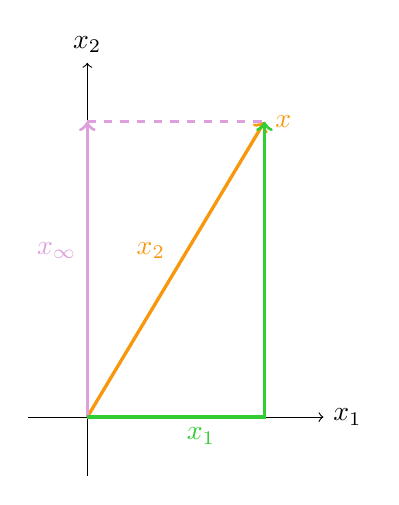
\begin{tikzpicture}[scale=1.5]
        % Draw axes
        \draw[->] (-0.5,0) -- (2,0) node[right] {$x_1$};
        \draw[->] (0,-0.5) -- (0,3) node[above] {$x_2$};
        % Draw vectors
        \draw[->, very thick, color=YellowOrange] (0,0) -- node[above left] {$\norm{x}_2$} ++(1.5,2.5) node[right] {$x$};
        \draw[->, very thick, color=Plum] (0,0) -- node[above left] {$\norm{x}_\infty$} ++(0,2.5) {};
        \draw[dashed, very thick, color=Plum] (0,2.5) -- (1.5,2.5) {};
        \draw[->, very thick, color=LimeGreen] (0,0) -- node[below right] {$\norm{x}_1$} ++(1.5,0) -- (1.5,2.5) {};
        % Draw norms
    \end{tikzpicture}
\end{center}

然而,从拓扑学的角度来说,这些度量并没有本质的区别,这是因为:

\begin{proposition}\label{prop:lp-metric}
    设$1\leq p\leq q\leq \infty$,则存在正常数$c_{p,q}$和$C_{p,q}$,对任意$x,y\in\R^n$,
    \[c_{p,q}\norm{x}_q\leq \norm{x}_p\leq C_{p,q}\norm{x}_q.\]
\end{proposition}
这一证明也依赖于H\"older不等式,所以也略去. 这一命题说明,虽然不同的范数对应的度量不同,但是他们之间的关系是最多差个常数倍. 我们后面会看到,这一性质表明$L^p$范数定义的所有拓扑性质都是完全相同的. 这一性质也可以一般化:

\begin{definition}[等价范数]\index{范数!等价~}
    设$X$是一个向量空间,$\norm{\cdot}_1$和$\norm{\cdot}_2$是$X$上的两个范数,如果存在正常数$c,C$,使得对任意$x\in X$,有
    \[c\norm{x}_1\leq \norm{x}_2\leq C\norm{x}_1,\]
    则称$\norm{\cdot}_1$和$\norm{\cdot}_2$是\textbf{等价}的. 
\end{definition}

\subsection{开集与闭集}
接下来我们进一步进行讨论$\R^n$空间的拓扑性质. 拓扑学是关于开集的学问,给定所有的开集,我们就可以研究一个空间的拓扑性质. 

在$\R$中,很早就已经有了\emph{开区间}的概念,它指的是集合$(a,b)=\{x\in\R:a<x<b\}$. 实际上,$\R$中的开集定义很简单,就是若干开区间的并集. 在更一般的拓扑空间中,开集的定义也是如此. 我们将视角聚焦在度量空间中. 我们可以把开区间$(a,b)$看成一个圆心在$(a+b)/2$,半径为$(b-a)/2$的一维开球. 从这个视角看,开集的定义是从开球给出的. 这样的定义是有一般性的:

\begin{definition}[开球,开集,拓扑空间]\index{开球}\index{开集}\index{拓扑空间}
    设$(X,d)$是一个度量空间,$x\in X$,$r>0$,定义
    \[B(x,r)=\{y\in X:d(x,y)<r\}.\]
    则称$B(x,r)$是以$x$为球心,$r$为半径的\textbf{开球}. 
    
    集合$U\subseteq X$被称为\textbf{开集},如果它是若干开球的并集. 

    $X$连同它的所有开集,被称为\textbf{拓扑空间}\footnote{一般拓扑空间的定义是给出所有开集的集合,并要求他们满足某种封闭性,然而我们这里只关心度量空间,所以不具体给出这些封闭性条件了. }. 
\end{definition}
在通常的微积分教科书上,我们会看到另一种开集的定义,即开集是任意一点都可以找到一个开球包含在这个集合中. 这两种定义是等价的:

\begin{proposition}\label{prop:open-ball}
    设$(X,d)$是一个度量空间,$U\subseteq X$,则$U$是开集当且仅当对任意$x\in U$,存在$r>0$,使得$B(x,r)\subseteq U$.
\end{proposition}
\begin{proof}
   $\implies$:设$U$是开集,$x\in U$,$U=\bigcup_{i\in I}B(x_i,r_i)$,则存在$i\in I$,使得$x\in B(x_i,r_i)$,取$r=r_i-d(x,x_i)$,显然$r>0$,并且$B(x,r)\subseteq B(x_i,r_i)\subseteq U$.

    $\impliedby$:设对任意$x\in U$,存在$r_x>0$,使得$B(x,r_x)\subseteq U$,则$U=\bigcup_{x\in U}B(x,r_x)$,是开集. 
\end{proof}
我们给的定义是一个更拓扑、更整体的定义:开集就是由基本的开集(开球)经过任意次的并得到的集合,这一定义关心的集合而不是具体的元素. 而等价的定义,我们称之为点定义,是更局部的定义,这一定义关心的是点而不是集合. 今后的定义,我们都尝试用两种方式给出,特别地,拓扑的定义只使用开集而不使用度量. 


我们给几个开集的例子:
\begin{example}[范等价拓扑空间]
    设$X$是一个线性空间,它上面有两个等价的范数$\norm{\cdot}_1$和$\norm{\cdot}_2$\footnote{注意,对一般空间来说,这样的记号不意味着$L^1$或者$L^2$范数. },则两个赋范空间$(X,\norm{\cdot}_1)$和$(X,\norm{\cdot}_2)$定义了相同的拓扑空间. 因此,在拓扑意义下,$\R^n$空间到底装备了哪个$L^p$范数是不重要的,因此对于同一个数学对象(集合、序列、函数)来说,收敛性、完备性以及连续性在$L^p$范数下都是完全一样的. 

    事实上,设$U$是$(X,\norm{\cdot}_1)$中的开集,$x\in U$,则存在$r>0$,使得$B_1(x,r)\subseteq U$,由范数等价,存在$c,C>0$,使得$c\norm{x}_2\leq \norm{x}_1\leq C\norm{x}_2$,则$B_2(x,r/c)\subseteq B_1(x,r)\subseteq U$,所以$U$是$(X,\norm{\cdot}_2)$中的开集. 反之亦然. 
\end{example}

\begin{example}[乘积拓扑空间]\label{ex:product-topology}
    设$(X_1,d_1)$和$(X_2,d_2)$是两个度量空间,则$X_1\times X_2$上的开集有两种方式给出:
    \begin{enumerate}
        \item 规定$X_1\times X_2$上的度量$d$,然后利用这个度量给出开集;
        \item 对任意开集$U_1\subseteq X_1$和$U_2\subseteq X_2$,定义$U_1\times U_2$,则$U_1\times U_2$是$X_1\times X_2$上的开集,然后利用这些基本的开集给出所有开集. 
    \end{enumerate}
    如果我们把度量$d$定义为
    \[d((x_1,y_1),(x_2,y_2))=\norm{(d_1(x_1,x_2),d_2(y_1,y_2))}.\]
    其中$\norm{\cdot}$是$\R^2$的某个$L^p$范数,可以证明,这两种方式给出的$X_1\times X_2$上的拓扑完全相同. 因此,以后出现带有“拓扑空间$X\times Y$”这暗示的地方,所指的拓扑空间都是由这两种等价方式给出的. 这一结论可以推广到任意有限个度量空间的乘积. 
\end{example}

开集的重要性质是:

\begin{proposition}\label{prop:open-prop}
    设$(X,d)$是一个非空度量空间,则
    \begin{enumerate}
        \item $X$和$\varnothing$是开集;
        \item 任意个开集的并集是开集;
        \item 有限个开集的交集是开集. 
    \end{enumerate}
\end{proposition}
\begin{proof}
\begin{enumerate}
    \item 取$x\in X$,则$X=\bigcup_{r>0}B(x,r)$,是开集. $\varnothing$是零个(也是若干个)开集的并集,是开集. 

    \item 设$\{U_i\}_{i\in I}$是一族开集,$U_i=\bigcup_{j\in J_i} B(x_j,r_j)$,显然$U=\bigcup_{i\in I}U_i=\bigcup_{i\in I,j\in J_i} B(x_j,r_j)$,是开集. 

    \item 设$U_1,\dots,U_n$是开集,$U=\bigcap_{i=1}^nU_i$,对任意$x\in U$,对任意$i=1,\dots,n$,$x\in U_i$,由开集的点定义,存在$r_i>0$,使得$B(x,r_i)\subseteq U_i$,取$r=\min_{i=1}^n r_i$,则$B(x,r)\subseteq U_i$,所以$U$是开集. 
\end{enumerate}
\end{proof}
注意,开集只对有限交封闭. 可以看一个简单的例子:$\bigcap_{n=1}^\infty(-1/n,1/n)=\{0\}$,但是$\{0\}$不是开集,因为这个集合不可能包含任何开球. 

与开集相对应的是闭集的概念. 闭集的定义是:

\begin{definition}[闭集]\index{闭集}
    设$(X,d)$是一个度量空间,$F\subseteq X$,如果$X\setminus F$是开集,则称$F$是\textbf{闭集}. 
\end{definition}
闭集的定义是开集的对偶,所以有如下性质:

\begin{proposition}\label{prop:closed-prop}
    设$(X,d)$是一个非空度量空间,则
    \begin{enumerate}
        \item $X$和$\varnothing$是闭集;
        \item 任意个闭集的交集是闭集;
        \item 有限个闭集的并集是闭集. 
    \end{enumerate}
\end{proposition}

需要注意的是,开集似乎可以简单理解为开区间的推广,然而闭集完全不是这样的,闭集是把若干开区间挖出来得到的集合,并不是闭区间的简单推广,所以比起把开区间拼起来会复杂得多,例如Cantor集就是一个性质非常奇怪的闭集. 

\subsection{紧集,收敛性,完备性}

接下来我们讨论一个更微妙的概念,\emph{紧集}. 紧性与极限、收敛、连续等概念有着密切的联系,然而如何恰当的定义紧性是一个很难的问题. 我们这里不讨论历史,只给出历史的答案. 简单来说,\emph{紧}这个词的概念是\emph{压缩},将无穷多的东西变成有限个. 我们的逻辑推理通常只能处理有限的东西,所以紧性是沟通无穷和有限的桥梁. 下面给出紧集的定义:

\begin{definition}[开覆盖,紧集]\index{开覆盖}\index{紧集}
    设$(X,d)$是一个度量空间,$F\subseteq X$,如果存在一族开集$\{U_i\}_{i\in I}$,使得$F\subseteq \bigcup_{i\in I}U_i$,则称$\{U_i\}_{i\in I}$是$F$的一个\textbf{开覆盖}. 
    
    如果对任意$F$的开覆盖$\{U_i\}_{i\in I}$,都存在有限子覆盖$\{U_{i_j}\}_{j=1}^n$,使得$F\subseteq \bigcup_{j=1}^nU_{i_j}$,则称$F$是\textbf{紧集}. 
\end{definition}
这当然是一个非常抽象的定义. 然而,我们没有办法将它还原为更直观的定义了. 例如,即便在最基本的集合$\R$上,紧集的存在性也只能被作为与实数公理\footnote{当然,这样的说法把实数集作为一个数学对象,试图用公理定义出来,而不是从已有的数学对象构造出来(例如Dedekind分割). }等价的命题存在:

\begin{proposition}[Heine-Borel有限覆盖原理]\label{prop:heine-borel}
设$F$是$\R$的一个闭区间,对任意$F$开覆盖$\{U_i\}_{i\in I}$,存在有限子覆盖$\{U_{i_j}\}_{j=1}^n$.
\end{proposition}
这一原理说明,闭区间是紧集,因而给出了紧集的存在性. 

在度量空间上,紧集与收敛性密切相关. 为此,我们需要形式地定义度量空间中的收敛概念. 我们先使用$\epsilon-N$语言定义:

\begin{definition}[收敛,极限]\index{收敛}\index{极限}
    设$(X,d)$是一个度量空间,$\{x_n\}_{n=1}^\infty$是$X$中的一个序列,$x\in X$,如果对任意$\epsilon>0$,存在$N\in\N$,使得对任意$n>N$,$d(x_n,x)<\epsilon$,则称$\{x_n\}_{n=1}^\infty$收敛到$x$,记作$\lim_{n\to\infty}x_n=x$或$x_n\to x$,$n\to\infty$,$x$称为$\{x_n\}_{n=1}^\infty$的\textbf{极限}. 
\end{definition}
直观上说,这一定义在刻画一列点越来越接近某个点$x$. 如果我们将定义中的$N$取掉,这一直观会更清楚:对任意$\epsilon>0$,除掉有限个$n$(也就是前$N$个),都有$x_n\in B(x,\epsilon)$. 所谓越来越接近,指的就是画任意一个球$B(x,\epsilon)$,除去有限个$x_n$,剩下的所有$x_n$都在这个球里面. 这一想法给出了只基于开集的等价定义:

\begin{proposition}\label{prop:converge-ball}
    设$(X,d)$是一个度量空间,$\{x_n\}_{n=1}^\infty$是$X$中的一个序列,$x\in X$,则$\{x_n\}_{n=1}^\infty$收敛到$x$当且仅当对任意包含$x$的开集$U$,存在$N\in\N$,使得对任意$n>N$,$x_n\in U$.
\end{proposition}
\begin{proof}
    $\implies$:设$\{x_n\}_{n=1}^\infty$收敛到$x$,$U$是包含$x$的开集,由开集的点定义,存在$r>0$,使得$B(x,r)\subseteq U$,由收敛的定义,存在$N\in\N$,使得对任意$n>N$,$d(x_n,x)<r$,所以$x_n\in B(x,r)\subseteq U$.

    $\impliedby$:设对任意包含$x$的开集$U$,存在$N\in\N$,使得对任意$n>N$,$x_n\in U$,则对任意$\epsilon>0$,取$U=B(x,\epsilon)$,则存在$N\in\N$,使得对任意$n>N$,$x_n\in B(x,\epsilon)$,即$d(x_n,x)<\epsilon$,所以$\{x_n\}_{n=1}^\infty$收敛到$x$.
\end{proof}
在更一般的拓扑空间中,甚至没有度量的概念,然而,开集定义收敛依然是可以的:这正是这一命题的意义. 

下面给一些收敛的经典例子:
\begin{example}
\begin{itemize}
    \item 在$\R$中,$\{1/n\}_{n=1}^\infty$收敛到$0$,然而,序列$\{n\}_{n=1}^\infty$则不收敛. 这个例子表明,极限未必需要在序列中出现,以及趋于无穷是一种特殊的不收敛.
    \item 在$\R^n$和$L^p$范数下,$\{x_n\}_{n=1}^\infty$收敛到$x$,当且仅当对任意$i=1,\dots,n$,$\{x_n^i\}_{n=1}^\infty$收敛到$x^i$. 这个例子表明,高维空间中的收敛性可以从每个分量看. 
    \item 在$C([0,1])$和$L^\infty$范数下,$f_n\to f$实际上是所谓\textbf{一致收敛}\index{收敛!一致~}的概念,即对任意$\epsilon>0$,存在不依赖$x$的$N\in\N$,使得对任意$n>N$,任意$x\in[0,1]$,$|f_n(x)-f(x)|<\epsilon$. 在这一概念下,$\{x^n\}_{n=1}^\infty$就不收敛(尽管它逐点收敛). 
\end{itemize}
\end{example}

度量空间中紧集可以完全由收敛性来刻画:

\begin{theorem}\label{thm:compact-converge}
    设$(X,d)$是一个度量空间,$F\subseteq X$,则$F$是紧集当且仅当$F$中的任意序列都有收敛子列. 
\end{theorem}
这一定理的证明并不算困难,但是需要陈述的事实较多,且与本书关联不大,所以这里都略去. 

这一定理足以表明紧集这一概念的重要性了,然而,这一定理的成立只需要度量空间,度量空间是一个非常弱的概念,我们关心的$\R^n$空间实际上有更强的性质,这一性质是完备性. 要定义完备性,我们需要Cauchy列. 

\begin{definition}[Cauchy列]\index{Cauchy列}
    设$(X,d)$是一个度量空间,$\{x_n\}_{n=1}^\infty$是$X$中的一个序列,如果对任意$\epsilon>0$,存在$N\in\N$,使得对任意$m,n>N$,$d(x_m,x_n)<\epsilon$,则称$\{x_n\}_{n=1}^\infty$是一个\textbf{Cauchy列}. 
\end{definition}

Cauchy列描述了另一种收敛的概念,它要求的是序列中的点越来越相互接近,而不是越来越接近某个点. 注意,这一定义没有办法像收敛性一样给一个纯拓扑的定义,所以Cauchy列的概念是依赖于度量的. 自然,收敛的点列是Cauchy列:

\begin{proposition}\label{prop:cauchy-converge}
    设$(X,d)$是一个度量空间,$\{x_n\}_{n=1}^\infty$是$X$中的一个序列,如果$\{x_n\}_{n=1}^\infty$收敛,则$\{x_n\}_{n=1}^\infty$是Cauchy列. 
\end{proposition}
\begin{proof}
    设$\{x_n\}_{n=1}^\infty$收敛到$x$,则对任意$\epsilon>0$,存在$N\in\N$,使得对任意$n>N$,$d(x_n,x)<\epsilon/2$,所以对任意$m,n>N$,$d(x_m,x_n)\leq d(x_m,x)+d(x,x_n)<\epsilon$,所以$\{x_n\}_{n=1}^\infty$是Cauchy列. 
\end{proof}

反过来,Cauchy列是否一定收敛呢?这一问题的答案是不一定. 实际上,在$\R$上,就如同有限覆盖原理,这件事情的成立只能作为与实数公理等价的命题存在!完备性指的就是Cauchy列一定收敛的性质:

\begin{definition}[完备度量空间]\index{完备度量空间}
    设$(X,d)$是一个度量空间,如果$X$中的任意Cauchy列都收敛,则称$(X,d)$是一个\textbf{完备度量空间}. 
\end{definition}
我们不加证明地给出完备度量空间的例子:
\begin{example}
\begin{itemize}
\item 有限维空间的例子:$L^p$范数下$\R^n$是完备的.
\item 反面的例子:使用度量$d(x_1,x_2)=|x_1-x_2|$,则$X=\R\setminus\{0\}$不是完备度量空间. 考虑$\{x_n=\frac1n:n\in\N\}$,它是Cauchy列,但该点列在$X$中没有极限(极限是$0$).
\item 无穷维空间的的例子:$[0,1]$到自身的连续函数空间$C([0,1])$在$L^\infty$范数下是完备的.
\item 无穷维空间的另一个例子:$\ell^p$空间是完备的. 
\end{itemize}
\end{example}

最后我们指出,尽管完备度量空间已经足够发展微积分了,但是它和$\R^n$依然有一个本质的区别,这一区别在于紧集. 首先,在有限维情况下,紧集与有界闭集是等价的:

\begin{proposition}\label{prop:compact-bounded}
设$\R^n$装备了$L^p$范数,设$F\subseteq\R^n$,那么$F$是紧集当且仅当$F$是有界闭集,有界指的是存在$M>0$,使得对任意$x\in F$,$\norm{x}_p\leq M$.
\end{proposition}
这一命题的证明依赖于Heine-Borel有限覆盖原理,这里就不给出细节了. 然而,在无穷维空间中,这一命题不一定成立:

\begin{proposition}\label{prop:compact-not-bounded}
考虑$\ell^2$的标准正交基$\{e_i\}_{i=1}^\infty$,考虑单位球面$E=\{x\in\ell^2:\norm{x}_2=1\}$,则$E$是有界闭集,但不是紧集. 
\end{proposition}
\begin{proof}
    因为对任意$x\in E$,$\norm{x}=1$,所以$\norm{x}_2\leq 1$,所以$E$是有界集. 取$x\in\ell^2\setminus E$. 如果$\norm{x}=r<1$,那么开球$B(x,(1-r)/2)\subseteq B(0,1)\subseteq \ell^2\setminus E$;对于$r>1$可以同理讨论. 这就证明了$E$是闭集. 最后证明$E$不是紧集. 考虑序列$\{e_i\}_{i=1}^\infty$,它是$E$中的序列,因为对任意不同的$m,n$,$\norm{e_m-e_n}=2$,因此$\{e_i\}$的任何子列都不是Cauchy列,根据\Cref{prop:cauchy-converge} 的逆否命题,$\{e_i\}$没有任何收敛子列,因而根据\Cref{thm:compact-converge},$E$不是紧集. 
\end{proof}

\subsection{连续映射}
接下来我们讨论两个拓扑空间之间的映射. 我们说过,拓扑空间完全由开集给出,所以某种程度保持拓扑性质的映射也会与开集有关系. 对于微积分来说,连续性是其中最重要的一种. 遵循先前的惯例,我们先给出更像微积分的$\delta$-$\epsilon$语言的点定义,然后再给出更像拓扑的定义. 

$\delta$-$\epsilon$语言的定义实际上给出了\emph{映射的极限}这一概念:

\begin{definition}[映射的极限]\index{极限}
    设$(X,d_X)$和$(Y,d_Y)$是两个度量空间,$f:X\to Y$是一个映射,$x_0\in X$,$y\in Y$,如果对任意$\epsilon>0$,存在$\delta>0$,使得对任意$x\in X$,如果$0<d_X(x,x_0)<\delta$,则$d_Y(f(x),y)<\epsilon$,则称$y$是$f$在$x_0$处的\textbf{极限},记作$\lim_{x\to x_0}f(x)=y$或$f(x)\to y$,$x\to x_0$.
\end{definition}
注意到,定义中我们实际上划定了$x$的范围,即$x\neq x_0$,或者说去心邻域$B(x_0,\delta)\setminus\{x_0\}$,这样做允许极限并不等于$f(x_0)$本身。

\begin{remark}
映射的极限还可以定义自变量趋于无穷、单侧极限以及其他情况,我们后面会使用这些概念,他们的直观含义都是明确的,这里我们不再给出正式定义,我们只给出他们的记号:
\begin{itemize}
    \item 趋于无穷:$\lim_{x\to\infty}f(x)=y$或$f(x)\to y$,$x\to\infty$;
    \item 如果定义域是$\R$,还可以定义趋于正、负无穷:$\lim_{x\to+\infty}f(x)=y$或$f(x)\to y$,$x\to+\infty$,$\lim_{x\to-\infty}f(x)=y$或$f(x)\to y$,$x\to-\infty$;
    \item 单调递增趋于:$x\uparrow x_0$,单调递减趋于:$x\downarrow x_0$。这些记号既可以出现在自变量中,也可以出现在函数值中,例如我们可以写$n/(n+1)\uparrow 1$,$n\to\infty$.
    \item 如果定义域是$\R$,还可以定义单侧极限,从负向趋于某点(左极限):$\lim_{x\uparrow x_0}f(x)=y$或$f(x)\to y$,$x\uparrow x_0$,以及从正向趋于某点(右极限):$\lim_{x\downarrow x_0}f(x)=y$或$f(x)\to y$,$x\downarrow x_0$.
\end{itemize}
\end{remark}

由此,我们可以定义连续映射:
\begin{definition}[连续映射]\index{连续映射}
    设$(X,d_X)$和$(Y,d_Y)$是两个度量空间,$f:X\to Y$是一个映射,考虑点$x\in X$,如果对任意$y\in Y$,如果$\lim_{x\to x'}f(x)=y$,则称$f$在$x$处\textbf{连续},如果$f$在$X$的每一点都连续,则称$f$是\textbf{连续映射}.
\end{definition}

直观上说,连续映射是指,$x$和$y$足够接近的时候$f(x)$和$f(y)$也足够接近. 然而,数学定义其实是反过来的:想让$f(x)$和$f(y)$足够接近,我们只需要让$x$和$y$足够接近. 更精确一些来说,如果我们画了一个$f(x)$的任意小的范围,我们只需要找到一个$x$的范围,使得$x$的范围里的点都被映射到$f(x)$的范围里. 这一定义可以用开集来表述,为此,我们需要先引入一些关于映射的概念. 

\begin{definition}[像,原像]\index{像}\index{原像}
    设$f:X\to Y$是一个映射,$A\subseteq X$,则$f(A)=\{f(x):x\in A\}$称为$A$的\textbf{像},如果$B\subseteq Y$,则$f^{-1}(B)=\{x\in X:f(x)\in B\}$称为$B$的\textbf{原像}. 
\end{definition}

于是,我们可以用开集表述极限和连续性了:

\begin{proposition}\label{prop:continuous-open}
    设$(X,d_X)$和$(Y,d_Y)$是两个度量空间,$f:X\to Y$是一个映射,则
\begin{enumerate}
    \item $\lim_{x\to x_0} f(x)=y$当且仅当对任意包含$y$的开集$U\subseteq Y$,存在包含$x_0$的开集$V\subseteq X$,使得$f(V\setminus\{x_0\})\subseteq U$;
    \item  $f$在$x\in X$处连续当且仅当对任意包含$f(x)$的开集$U\subseteq Y$,存在包含$x$的开集$V\subseteq X$,使得$f(V)\subseteq U$.
\end{enumerate}
\end{proposition}
这一命题的证明非常类似\Cref{prop:open-ball},我们这里就不给出了. 注意,极限的开集定义所用的集合$V\setminus\{x_0\}$也是一个开集,它是$x_0$的去心邻域。连续映射的定义也可以完全由拓扑给出:

\begin{proposition}\label{prop:continuous-topology}
    设$(X,d_X)$和$(Y,d_Y)$是两个度量空间,$f:X\to Y$是一个映射,则下列表述等价:
    \begin{enumerate}
        \item $f$是连续映射;
        \item 对任意$Y$中的开集$U$,原像$f^{-1}(U)$是$X$中的开集;
        \item 对任意$Y$中的闭集$F$,原像$f^{-1}(F)$是$X$中的闭集. 
    \end{enumerate}
\end{proposition}
利用\Cref{prop:continuous-open}、\Cref{prop:closed-prop} 以及开集的定义,很容易证明这一命题,我们就不再证明了. 

\begin{example}
在不给任何额外定义的时候,我们有一个非常自然的连续函数的例子,那就是\textbf{度量}. 设$(X,d)$是一个度量空间,我们证明度量$d:X\times X\to\R$是一个连续函数. 

我们利用点连续的定义,证明$d$在每一点都连续. 设$(x_1,y_1)\in X\times X$. 我们利用\Cref{prop:continuous-open} 和原始定义的混合版本. 注意到要证明所有包含$d_0=d(x_1,y_1)$的开集$U$满足条件,根据$U$的构造,只需要证明,对任意$\epsilon>0$,$B(d_0,\epsilon)$满足条件. 为此,取一个包含$(x_1,y_1)$的开集$V=B(x_1,\epsilon/2)\times B(y_1,\epsilon/2)$(关于这个为什么是开集,详细讨论见\Cref{ex:product-topology}),则对任意$(x_2,y_2)\in V$,有$d(x_1,x_2)<\epsilon/2$,$d(y_1,y_2)<\epsilon/2$,所以根据三角不等式,
\[d(x_2,y_2)\leq d(x_1,y_1)+d(x_1,x_2)+d(y_1,y_2)<d_0+\epsilon/2+\epsilon/2=d_0+\epsilon.\]
另一方面,
\begin{align*}
    &d_0=d(x_1,y_1)\leq d(x_2,y_2)+d(x_1,x_2)+d(y_2,y_1)<d(x_2,y_2)+\epsilon\\
\implies& d(x_2,y_2)>d_0-\epsilon.
\end{align*}
所以,$d(x_2,y_2)\in B(d_0,\epsilon)$,即$V\subseteq B(d_0,\epsilon)$,所以$d$在$(x_1,y_1)$连续. 因为$(x_1,y_1)$是任意的,所以$d$是连续的.
\end{example}

连续性的定义实际分为了两部分,一个是局部的、点的连续性,另一个是整体的、只依赖开集而不依赖具体点的定义. 他们也对应了连续不同的性质. 我们首先讨论局部连续的性质,以下命题我们都不再给出证明. 

首先,极限也可以用收敛性刻画:

\begin{proposition}\label{prop:limit-converge}
    设$(X,d_X)$和$(Y,d_Y)$是两个度量空间,$f:X\to Y$是一个映射,$x_0\in X$,$y\in Y$,则下列表述等价:
    \begin{enumerate}
        \item $\lim_{x\to x_0}f(x)=y$;
        \item 对任意$\{x_n\}_{n=1}^\infty$,如果$x_n\to x_0$,则$f(x_n)\to y$.
    \end{enumerate}
\end{proposition}

利用这一条,很快就可以得到连续的序列版本:

\begin{corollary}\label{cor:continuous-converge}
    设$(X,d_X)$和$(Y,d_Y)$是两个度量空间,$f:X\to Y$是一个映射,则下列表述等价:
    \begin{enumerate}
        \item $f$是连续映射;
        \item 对任意$x\in X$,对任意$\{x_n\}_{n=1}^\infty$,如果$x_n\to x$,则$f(x_n)\to f(x)$.
    \end{enumerate}
\end{corollary}

其次,连续对复合是封闭的:
\begin{proposition}\label{prop:continuous-composition}
    设$(X,d_X)$、$(Y,d_Y)$和$(Z,d_Z)$是三个度量空间,$f:X\to Y$在$x\in X$连续,$g:Y\to Z$在$f(x)\in Y$连续,则$g\circ f:X\to Z$在$x$连续. 
\end{proposition}

利用以上两个性质,在赋范空间中,我们得到如下结论:
\begin{corollary}\label{cor:continuous-linear}
    设$(X,\norm{\cdot}_X)$是赋范空间,则数乘是$X\to X$的连续映射,向量加法是$X\times X\to X$的连续映射. 因此,有限维线性空间到有限维线性空间的线性映射都是连续映射. 
\end{corollary}
根据\Cref{cor:continuous-converge},这一结论也有对应的序列版本,我们就不再列出了. 特别要注意的是,这一结论也适用于$\R$,从数乘来看,对于$\R$来说,乘法$\times:\R\times\R\to\R$和除法$\div:\R\times(\R\setminus\{0\})\to\R$也都是连续映射\footnote{尽管从证明的逻辑顺序来说,应该是先有了实数的四则运算连续性,然后才有了赋范空间的连续性. 我们这样写是为了避免不必要的冗余,直接从一个一般的视角出发来讨论. }. 

最后,连续意味着有界:
\begin{proposition}\label{prop:continuous-bounded}
    设$(X,d_X)$和$(Y,d_Y)$是两个度量空间,$f:X\to Y$在$x\in X$连续,则在$x$的某个邻域上$f$有界,即存在$r,M>0$,对任意$y\in B(f(x),r)$,有$d_Y(f(x),y)\leq M$. 
\end{proposition}

接下来我们讨论连续映射整体的性质,这些性质都与紧集有关. 首先,连续映射将紧集映射为紧集:

\begin{proposition}\label{prop:continuous-compact}
    设$(X,d_X)$和$(Y,d_Y)$是两个度量空间,$f:X\to Y$是一个连续映射,$F\subseteq X$是紧集,则$f(F)$是紧集. 
\end{proposition}

其他性质将在下一节给出。

\subsection{与实数有关的性质}

本节要讨论的性质都限制映射的值是实数,即$f:X\to \R$. 这样的映射我们称之为\emph{函数}. $\R^n$区别于$\R^n$最大的不同是实数可以比大小而实数向量不行,实数与大小相关的性质有很多,我们列出其中两个与实数公理等价的. 这些性质需要用到\emph{界}和\emph{确界}的概念,这一概念将会频繁出现在我们的讨论中,所以这里单独给出:

\begin{definition}[上界,上确界,下界,下确界]\index{上确界}\index{下确界}\index{上界}\index{下界}
    设$A\subseteq\R$,如果存在$M\in\R$,使得对任意$a\in A$,$a\leq M$,则称$M$是$A$的一个\textbf{上界},如果$M$是$A$的上界,且对任意$M'<M$,存在$a\in A$,使得$a>M'$,则称$M$是$A$的一个\textbf{上确界},记作$\sup A$. 
    
    类似地,如果存在$M\in\R$,使得对任意$a\in A$,$a\geq M$,则称$M$是$A$的一个\textbf{下界},如果$M$是$A$的下界,且对任意$M'>M$,存在$a\in A$,使得$a<M'$,则称$M$是$A$的一个\textbf{下确界},记作$\inf A$. 
    
    如果一个集合有上(下)界,则称这个集合\textbf{上(下)有界},如果它既有上界又有下界,则称这个集合\textbf{有界}. 
\end{definition}
上确界这个概念,直观上就是在说“最小可能的上界”,下确界也有类似的解读. 

现在我们就可以阐述这两个实数的性质了. 第一个是说单调有界的序列一定收敛. 

\begin{proposition}[单调有界原理]\label{prop:monotone-bounded}
    设$\{x_n\}$是一个单调有界的实数列,则$\{x_n\}$收敛. 
\end{proposition}

接下来一个是说有上(下)界的实数集一定有上(下)确界,即最小可能的上(下)界是一个确实存在的实数,这也是一种完备性的体现. 
\begin{proposition}[确界原理]\label{prop:supremum}
    设$A\subseteq\R$,如果$A$有上界,则$\sup A$存在;如果$A$有下界,则$\inf A$存在. 
\end{proposition}

确界原理给了一种求确界的方式:
\begin{proposition}\label{prop:supremum-epsilon}
    设$A\subseteq\R$,如果$A$有上界,则存在一列$\{a_n\}$,使得$a_n\in A$,且$\lim_{n\to\infty}a_n=\sup A$.
\end{proposition}
\begin{proof}
    设$M=\sup A$(由确界原理知$M$存在),对任意$n\in\N$,由$M-1/n$不是$A$的上界,存在$a_n\in A$,使得$M-1/n<a_n\leq M$. 根据极限的定义易知$\lim_{n\to\infty}a_n=M$.
\end{proof}

对于实值函数来说,我们还需要比较在极限情况下两个函数的\emph{渐进大小},这就是$o$和$\O$符号。我们先给出这一概念在序列上的定义:

\begin{definition}[阶,无穷小,等价]\index{阶}\index{无穷小}\index{等价}
    设$\{x_n\}_{n=1}^\infty$和$\{y_n\}_{n=1}^\infty$是两个序列,如果$\lim_{n\to\infty}\frac{x_n}{y_n}=0$,则称$\{x_n\}_{n=1}^\infty$是$\{y_n\}_{n=1}^\infty$的\textbf{高阶无穷小},记作$x_n=o(y_n)$;如果存在一个正常数$C$使得除去有限个$n$都有$|x_n|\leq C |y_n|$,则称$\{x_n\}_{n=1}^\infty$的\textbf{阶不高于}$\{y_n\}_{n=1}^\infty$,记作$x_n=\O(y_n)$.

    如果$x_n=\O(y_n)$且$y_n=\O(x_n)$,那么称$\{x_n\}_{n=1}^\infty$和$\{y_n\}_{n=1}^\infty$是\textbf{同阶}的. 如果进一步$\lim_{n\to\infty}\frac{x_n}{y_n}=1$,则称$\{x_n\}_{n=1}^\infty$和$\{y_n\}_{n=1}^\infty$是\textbf{等价}的,记作$x_n\sim y_n$.
\end{definition}
上述定义可以非常自然迁移到函数上,我们不再赘述。下面是一些例子:

\begin{example}
\begin{itemize}
    \item $n\to\infty$时,$n^2=o(2^n)$,$n^{1/n}\sim 1$,$n^2\sim n^2+\log n$.
    \item $x\to 0$时,$\sin x\sim x$,$1/x=o(1/x^2)$。
    \item $n\to\infty$时,$\sum_{k=1}^n\frac{1}{n}\sim\ln n$.
\end{itemize}
\end{example}

最后,我们回到连续的整体性质上来. 首先是Weierstrass最值定理:

\begin{theorem}[Weierstrass最值定理]\label{thm:weierstrass}
    紧集上的连续函数$f:F\to\R$在该紧集$F$的某个点取 最大(最小)值. 
\end{theorem}

然后是介值定理:
\begin{theorem}[介值定理]\label{thm:intermediate}
    设$f:[a,b]\to\R$是一个连续函数,$f(a)<f(b)$,则对任意$y\in(f(a),f(b))$,存在$x\in(a,b)$,使得$f(x)=y$.
\end{theorem}
实际上,介值定理成立并不需要区间$[a,b]$,任何一个连通的拓扑空间都可以,但是连通性的表述不是很直观,所以我们这里就不给出了. 


\section{一元函数的微分学}

接下来,我们进入微分学的部分,同样,我们先从最基本的一元函数的情况入手。

\subsection{导数与微分的定义}\index{导数}\index{微分}

从近似的角度来说,\emph{微分}或者\emph{导数}的概念,本身在描述在某个点函数的线性近似,因此微分和导数本身也是一个(线性)映射。在一元函数中,我们或许无法看出来这一点,但是在更加一般的微分学中,这样的观点非常重要。因此,即便在一元部分,我们也尝试将这样的观点引入。

考虑一个函数$f:\R\to\R$,和点$x_0\in\R$,我们希望找到一个线性映射$df_{x_0}:\R\to\R$,使得$f(x)$在$x_0$附近的行为很接近这线性映射,即

\[
    f(x)\approx f(x_0)+\d f_{x_0}(x-x_0).
\]
更精确来说,我们希望两边的误差是一个关于$x-x_0$的高阶无穷小:
\[
    f(x)=f(x_0)+\d f_{x_0}(x-x_0)+o(x-x_0).
\]
这一记号的含义可以通过一些变换看出来:
\begin{equation}
\d f_{x_0}(1)=\frac{f(x)-f(x_0)}{x-x_0}+o(1).\label{eq:df-1}
\end{equation}
注意$\d f_{x_0}(x)=kx$,所以左边就是$k$,而右边是割线的斜率。式 \eqref{eq:df-1} 的含义其实就是说$k$就是割线斜率的极限,直观上这就是切线的斜率,这就是导数的几何含义. 这一过程可以见下图:

\begin{center}
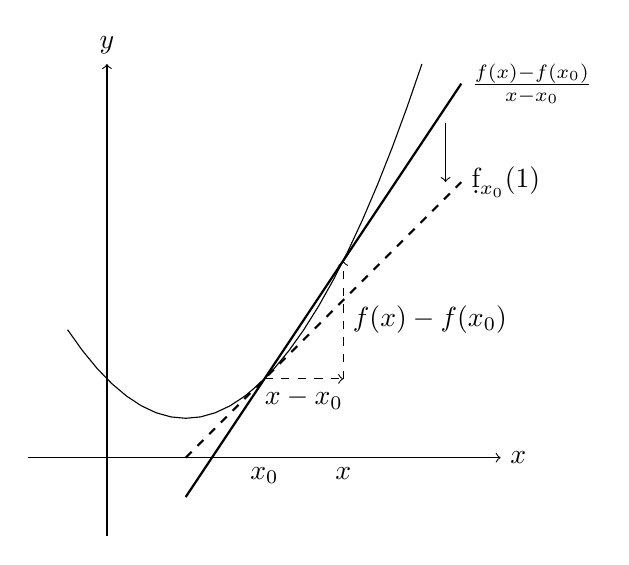
\begin{tikzpicture}
\draw[->] (-1,0) -- (5,0) node[right] {$x$};
\draw[->] (0,-1) -- (0,5) node[above] {$y$};
\draw[domain=-0.5:4] plot (\x,{0.5*\x*\x-\x+1});
\draw (2,0) node[below] {$x_0$};
\draw (3,0) node[below] {$x$};
\draw[dashed,->] (2,1) -- (3,1) node[midway,below] {$x-x_0$};
\draw[dashed,->] (3,1) -- (3,2.5) node[midway,right] {$f(x)-f(x_0)$};
\draw[thick] (2-1,1-1*1.5) -- (2+2.5,1+2.5*1.5) node[right] {$\frac{f(x)-f(x_0)}{x-x_0}$};
\draw[thick, dashed] (2-1,1-1) -- (2+2.5,1+2.5) node[right] {$\d f_{x_0}(1)$};
\draw[->] (2+2.3,1+2.3*1.5-0.2) -- (2+2.3,1+2.3+0.2) {};
\end{tikzpicture}
\end{center}

我们将这些讨论整理为如下定义:

\begin{definition}[微分,导数]\index{微分}\index{导数}
    设$f:\R\to\R$,$x_0\in\R$,如果存在一个线性映射$\d f_{x_0}:\R\to\R$,使得
    \[
        f(x)=f(x_0)+\d f_{x_0}(x-x_0)+o(x-x_0),
    \]
    则称$f$在$x_0$处\textbf{可微}或者\textbf{可导},$\d f_{x_0}$是$f$在$x_0$处的\textbf{微分}. 微分具有形式$\d f_{x_0}(x)=kx$,其中$k$称为$f$在$x_0$处的\textbf{导数},记作$f'(x_0)$.

    如果$f$在$\R$的每一点都可微,则称$f$是\textbf{可微}的或者\textbf{可导}的,$\d f$是$f$的\textbf{微分},$f'$是$f$的\textbf{导(函)数},也记作$\frac{\d f}{\d x}$或$\dot{f}$.
\end{definition}
关于导数的符号也有一些注。最能体现几何意义的是$\frac{\d f}{\d x}$,它是由Leibniz发明的。符号$\d$的意思就是“微”,可以理解为无穷小的变化量,所以导数就是自变量和函数值无穷小变化量的比值。另一方面,这个符号也可以理解为“切”,表示切向量的意思,例如$\d x$就是沿着$x$轴的任意切向量(实际上就是正方向或者负方向),而$\d y$就是相应地沿着$y$轴的切向量. 从这个角度来说,$\frac{\d f}{\d x}$就是$x$轴切向量到$y$轴切向量的一个线性映射。因此,微分其实就是所谓的\emph{切映射}\index{切映射},即从切向量到切向量的映射。这一视角在更抽象的微分学中是更本质的。

导数的定义也可以用更常见的形式给出:

\begin{proposition}\label{prop:derivative}
    设$f:\R\to\R$,$x_0\in\R$,那么$f$在$x_0$处可微当且仅当如下极限存在:
    \[
        \lim_{x\to x_0}\frac{f(x)-f(x_0)}{x-x_0}.
    \]
    这个极限就是$f$在$x_0$处的导数.
\end{proposition}

下面我们不加证明地列举导数的一些性质,这些性质自然也导出了微分的性质。

\begin{proposition}\label{prop:derivative-property}
    设$f,g:\R\to\R$在$x_0$处可微,则
    \begin{itemize}
        \item $f$在$x_0$处连续;
        \item $(f+g)'(x_0)=f'(x_0)+g'(x_0)$;
        \item $(fg)'(x_0)=f'(x_0)g(x_0)+f(x_0)g'(x_0)$;
        \item 如果$g(x_0)\neq 0$,则
        \[\left(\frac{f}{g}\right)'(x_0)=\frac{f'(x_0)g(x_0)-f(x_0)g'(x_0)}{g(x_0)^2};\]
        \item 链式法则:如果$f$在$x_0$处可微,$g$在$f(x_0)$处可微,则$g\circ f$在$x_0$处可微,且$(g\circ f)'(x_0)=g'(f(x_0))f'(x_0)$;
        \item 如果$f$存在反函数$f^{-1}$,则$f^{-1}$在$f(x_0)$处可微,且$(f^{-1})'(f(x_0))=\frac{1}{f'(x_0)}$.
    \end{itemize}
\end{proposition}
在Leibniz记号下,如果$z=z(y)$,$y=y(x)$,那么链式法则可以写作
\[
    \frac{\d z}{\d x}=\frac{\d z}{\d y}\cdot\frac{\d y}{\d x}.
\]
反函数的导数则可以写作
\[
    \frac{\d y}{\d x}=\left(\frac{\d x}{\d y}\right)^{-1}.
\]
我们再次看到这种记号的天才之处,它将复杂的计算简化为了一种直观的形式.

我们指出,链式法则和反函数求导法则在微分下有更加清晰的含义:

\begin{proposition}\label{prop:derivative-geometric}
设$f:\R\to\R$在$x_0$处可微,$g:\R\to\R$在$f(x_0)$处可微,则
\begin{itemize}
    \item $\d x=\id$;
    \item $\d(g\circ f)_{x_0}=\d g_{f(x_0)}\circ\d f_{x_0}$.
    \item  如果$f$存在反函数$f^{-1}$,则$\d(f^{-1})_{f(x_0)}=(\d f_{x_0})^{-1}$.
\end{itemize}
\end{proposition}

从这个意义上说,微分号$\d$相当于把$\R\to\R$的函数变成了另外一个$\R\to\R$的函数(即切映射),同时保持函数复合运算的单位元($\id$)、复合和逆元关系。利用这一性质,我们可以用更加代数的方法研究微分(微分函子),但这超出了本书的范围,我们就不再详细讨论了.

最后,我们讨论高阶导数的概念。高阶微分是一个相当抽象的概念,所以我们这里就不深入讨论了。我们只给出高阶导数的定义:

\begin{definition}[高阶导数]\index{导数}
    设$f:\R\to\R$,$x_0\in\R$,如果$f$在$x_0$处可微,则$f$在$x_0$处的导数$f'(x_0)$是一个实数. 如果$f'$在$x_0$处可微,则称$f$在$x_0$处\textbf{二阶可微},此时$f''(x_0)$是$f'$在$x_0$处的导数,称为$f$在$x_0$处的\textbf{二阶导数}. 一般地,如果$f^{(n-1)}$在$x_0$处可微,则称$f$在$x_0$处\textbf{$n$阶可微},此时$f^{(n)}(x_0)$是$f^{(n-1)}$在$x_0$处的导数,称为$f$在$x_0$处的\textbf{$n$阶导数}.
\end{definition}
在Leibniz的记号下,$n$阶导数可以写作
\[
    \frac{\d^n y}{\d x^n}=\underbrace{\frac{\d}{\d x}\cdots\frac{\d}{\d x}}_{n\text{个}}y.
\]
从这里我们可以看出,$\d/\d x$这个记号又仿佛是一个算子,它作用在函数上,得到一个新的函数,这个视角结合谱理论,发展出了非常重要的数学理论,成为了量子力学的基础。当然,这也不在本书的讨论范围之内了.

我们将在集合$X$上$n$次连续可微的函数的集合记作$C^n(X)$,任意次连续可微的函数的集合记作$C^\infty(X)$。

\section{微分学基本定理}

微分学几乎都与极值联系在一起,刻画这些关系的定理就是微分学的基本定理. 我们依然只罗列定理,不给出证明. 首先我们给出极值的定义。

\begin{definition}[极大值,严格极大值,极小值,严格极小值]\index{极值}
    设$f:X\to\R$,$x_0\in X$,如果存在包含$x_0$的开集$U$,使得对任意$x\in U$,有$f(x)\leq f(x_0)$,则称$f(x_0)$是$f$在$x_0$处的一个\textbf{极大值},$x_0$是$f$的一个\textbf{极大值点}。如果$f(x)=f(x_0)$只在$x_0$处成立,则称$f(x_0)$是$f$在$x_0$处的一个\textbf{严格极大值},$x_0$是$f$的一个\textbf{严格极大值点}.
    
    如果不等式反向,则称$f(x_0)$是$f$在$x_0$处的一个\textbf{极小值},$x_0$是$f$的一个\textbf{极小值点}. 如果$f(x)=f(x_0)$只在$x_0$处成立,则称$f(x_0)$是$f$在$x_0$处的一个\textbf{严格极小值},$x_0$是$f$的一个\textbf{严格极小值点}.
    
    如果$f(x_0)$是$f$在$x_0$处的一个极大(小)值,则称$f(x_0)$是$f$在$x_0$处的一个\textbf{极值},$x_0$是$f$的一个\textbf{极值点}. 
\end{definition}

首先是Fermat引理,他其实就是极值的一阶必要条件:

\begin{lemma}[Fermat引理]\label{lemma:fermat}
    设$f:X\to\R$,$x_0\in X$是$f$的一个极值点,且$f$在$x_0$处可微,则$f'(x_0)=0$.
\end{lemma}

接下来是一系列中值定理,我们这里只给出Lagrange中值定理:

\begin{theorem}[Lagrange中值定理]\label{thm:lagrange-mid}
    设$f:[a,b]\to\R$是一个连续函数,且在$(a,b)$内可微,则存在$\xi\in(a,b)$,使得
    \[
        f'(\xi)=\frac{f(b)-f(a)}{b-a}.
    \]
\end{theorem}

这一定理给出了割线斜率和切线斜率的关系,可以用下图来理解:

\begin{center}
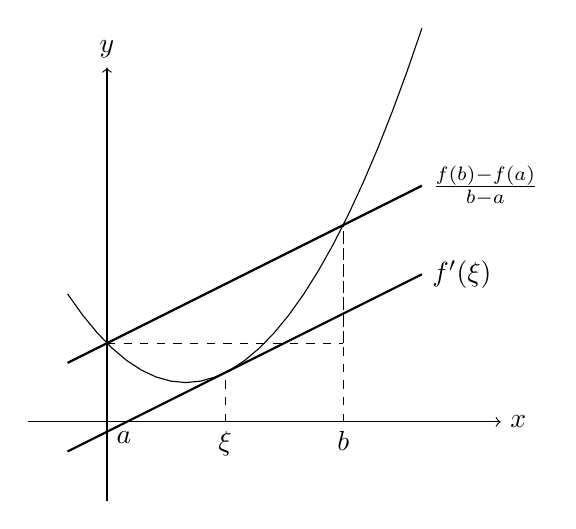
\begin{tikzpicture}
\draw[->] (-1,0) -- (5,0) node[right] {$x$};
\draw[->] (0,-1) -- (0,4.5) node[above] {$y$};
\draw[domain=-0.5:4] plot (\x,{0.5*\x*\x-\x+1});
\draw[dashed] (0,0) node[below right] {$a$} -- (0,1);
\draw[dashed] (3,0) node[below] {$b$} -- (3,2.5);
\draw[dashed] (0,1) -- (3,1) ;
\draw[dashed] (3,1) -- (3,2.5) ;
\draw[thick] (0-0.5,1-0.5*0.5) -- (0+4,1+4*0.5) node[right] {$\frac{f(b)-f(a)}{b-a}$};
\draw[dashed] (1.5,0) node[below] {$\xi$} -- (1.5,0.625);
\draw[thick] (1.5-2,0.625-2*0.5) -- (1.5+2.5,0.625+2.5*0.5) node[right] {$f'(\xi)$};
\end{tikzpicture}
\end{center}
我们将在后面指出,这一定理只适用于实值函数,假如想对向量值函数使用,需要对其进行适当的修改:

\begin{theorem}[Lagrange有限增量定理]\label{thm:lagrange-finite}
    设$f:[a,b]\to\R$是一个连续函数,且在$(a,b)$内可微,则
    \[
        |f(b)-f(a)|\leq |b-a|\sup_{\xi\in(a,b)}|f'(\xi)|.
    \]
\end{theorem}

接下来我们讨论高阶导数与极值的关系。这样的关系是由Taylor公式给出的。我们说过,微分是用线性函数去近似函数的过程,而Taylor公式则是用多项式去近似函数的过程。考虑函数$f:\R\to\R$,如果$f$在$x_0$处$n$次可微,我们尝试用一个$n$次多项式去近似$f$,即

\[
    f(x)=a_0+a_1(x-x_0)+\cdots+a_n(x-x_0)^n+o((x-x_0)^n).
\]
容易求出,$a_0=f(x_0)$,$a_1=f'(x_0)$,$a_2=\frac{f''(x_0)}{2}$,$a_3=\frac{f'''(x_0)}{6}$,$\cdots$,$a_k=\frac{f^{(k)}(x_0)}{n!}$,因此我们得到了Taylor公式:

\begin{theorem}
    设$f:\R\to\R$在$x_0$处$n$次可微,则
    \[
        f(x)=\sum_{k=0}^n\frac{f^{(k)}(x_0)}{k!}(x-x_0)^k+o((x-x_0)^n).
    \]
\end{theorem}
我们将这个$n$次多项式称为\textbf{Taylor展开}\index{Taylor展开}.

利用高阶导数,我们可以得到极值判定的充分条件:

\begin{theorem}\label{thm:extreme}
    设$f:(a,b)\to\R$在$x_0$处$n$次可微,且$f'(x_0)=f''(x_0)=\cdots=f^{(n-1)}(x_0)=0$,$f^{(n)}(x_0)\neq 0$,则
    \begin{itemize}
        \item 如果$n$为奇数,$f$在$x_0$处没有极值;
        \item 如果$n$为偶数,$f$在$x_0$处有极值,且当$f^{(n)}(x_0)>0$时,$f$在$x_0$处有严格极小值,当$f^{(n)}(x_0)<0$时,$f$在$x_0$处有严格极大值.
    \end{itemize}
\end{theorem}

\section{多元函数的微分学}

\section{线性赋范空间的微分学,矩阵微分学}
